% % !TEX root = ./presentation.tex 
\documentclass[presentation]{subfiles}

\begin{document}


\begin{frame}[t]{Scientific Forestry}

\textbf{People needed timber}

They were clamoring for ways to figure out how many trees they could cut down without doing irreparable harm.

\begin{columns}
\begin{column}{0.66\textwidth}

\only<2>{\includegraphics[width=\textwidth]{figures/zoom/1.png}}
\only<3>{\includegraphics[width=\textwidth]{figures/zoom/2.png}}
\only<4>{\includegraphics[width=\textwidth]{figures/zoom/3.png}}
\only<5>{\includegraphics[width=\textwidth]{figures/zoom/4.png}}
\only<6->{\includegraphics[width=\textwidth]{figures/zoom/5.png}}

\end{column}

\begin{column}{0.3\textwidth}
\vspace{-3em}


\visible<7>{
What about\dots
\begin{itemize}
  \item wildlife?
  \item people?
  \item other trees and flora?
\end{itemize}

}
\end{column}
\end{columns}

\end{frame}


\begin{frame}[standout]

Interpreting the world in a reductive way isn't wrong

\visible<2>{(It's how we cope with too much information)}

\end{frame}

\begin{frame}\frametitle{interpretation to imposition}
  

  \begin{columns}
  \begin{column}{0.6\textwidth}
  \centering
(imagine a picture of a forest here)
\end{column}
  \begin{column}{0.4\textwidth}
  \centering
  \only<2>{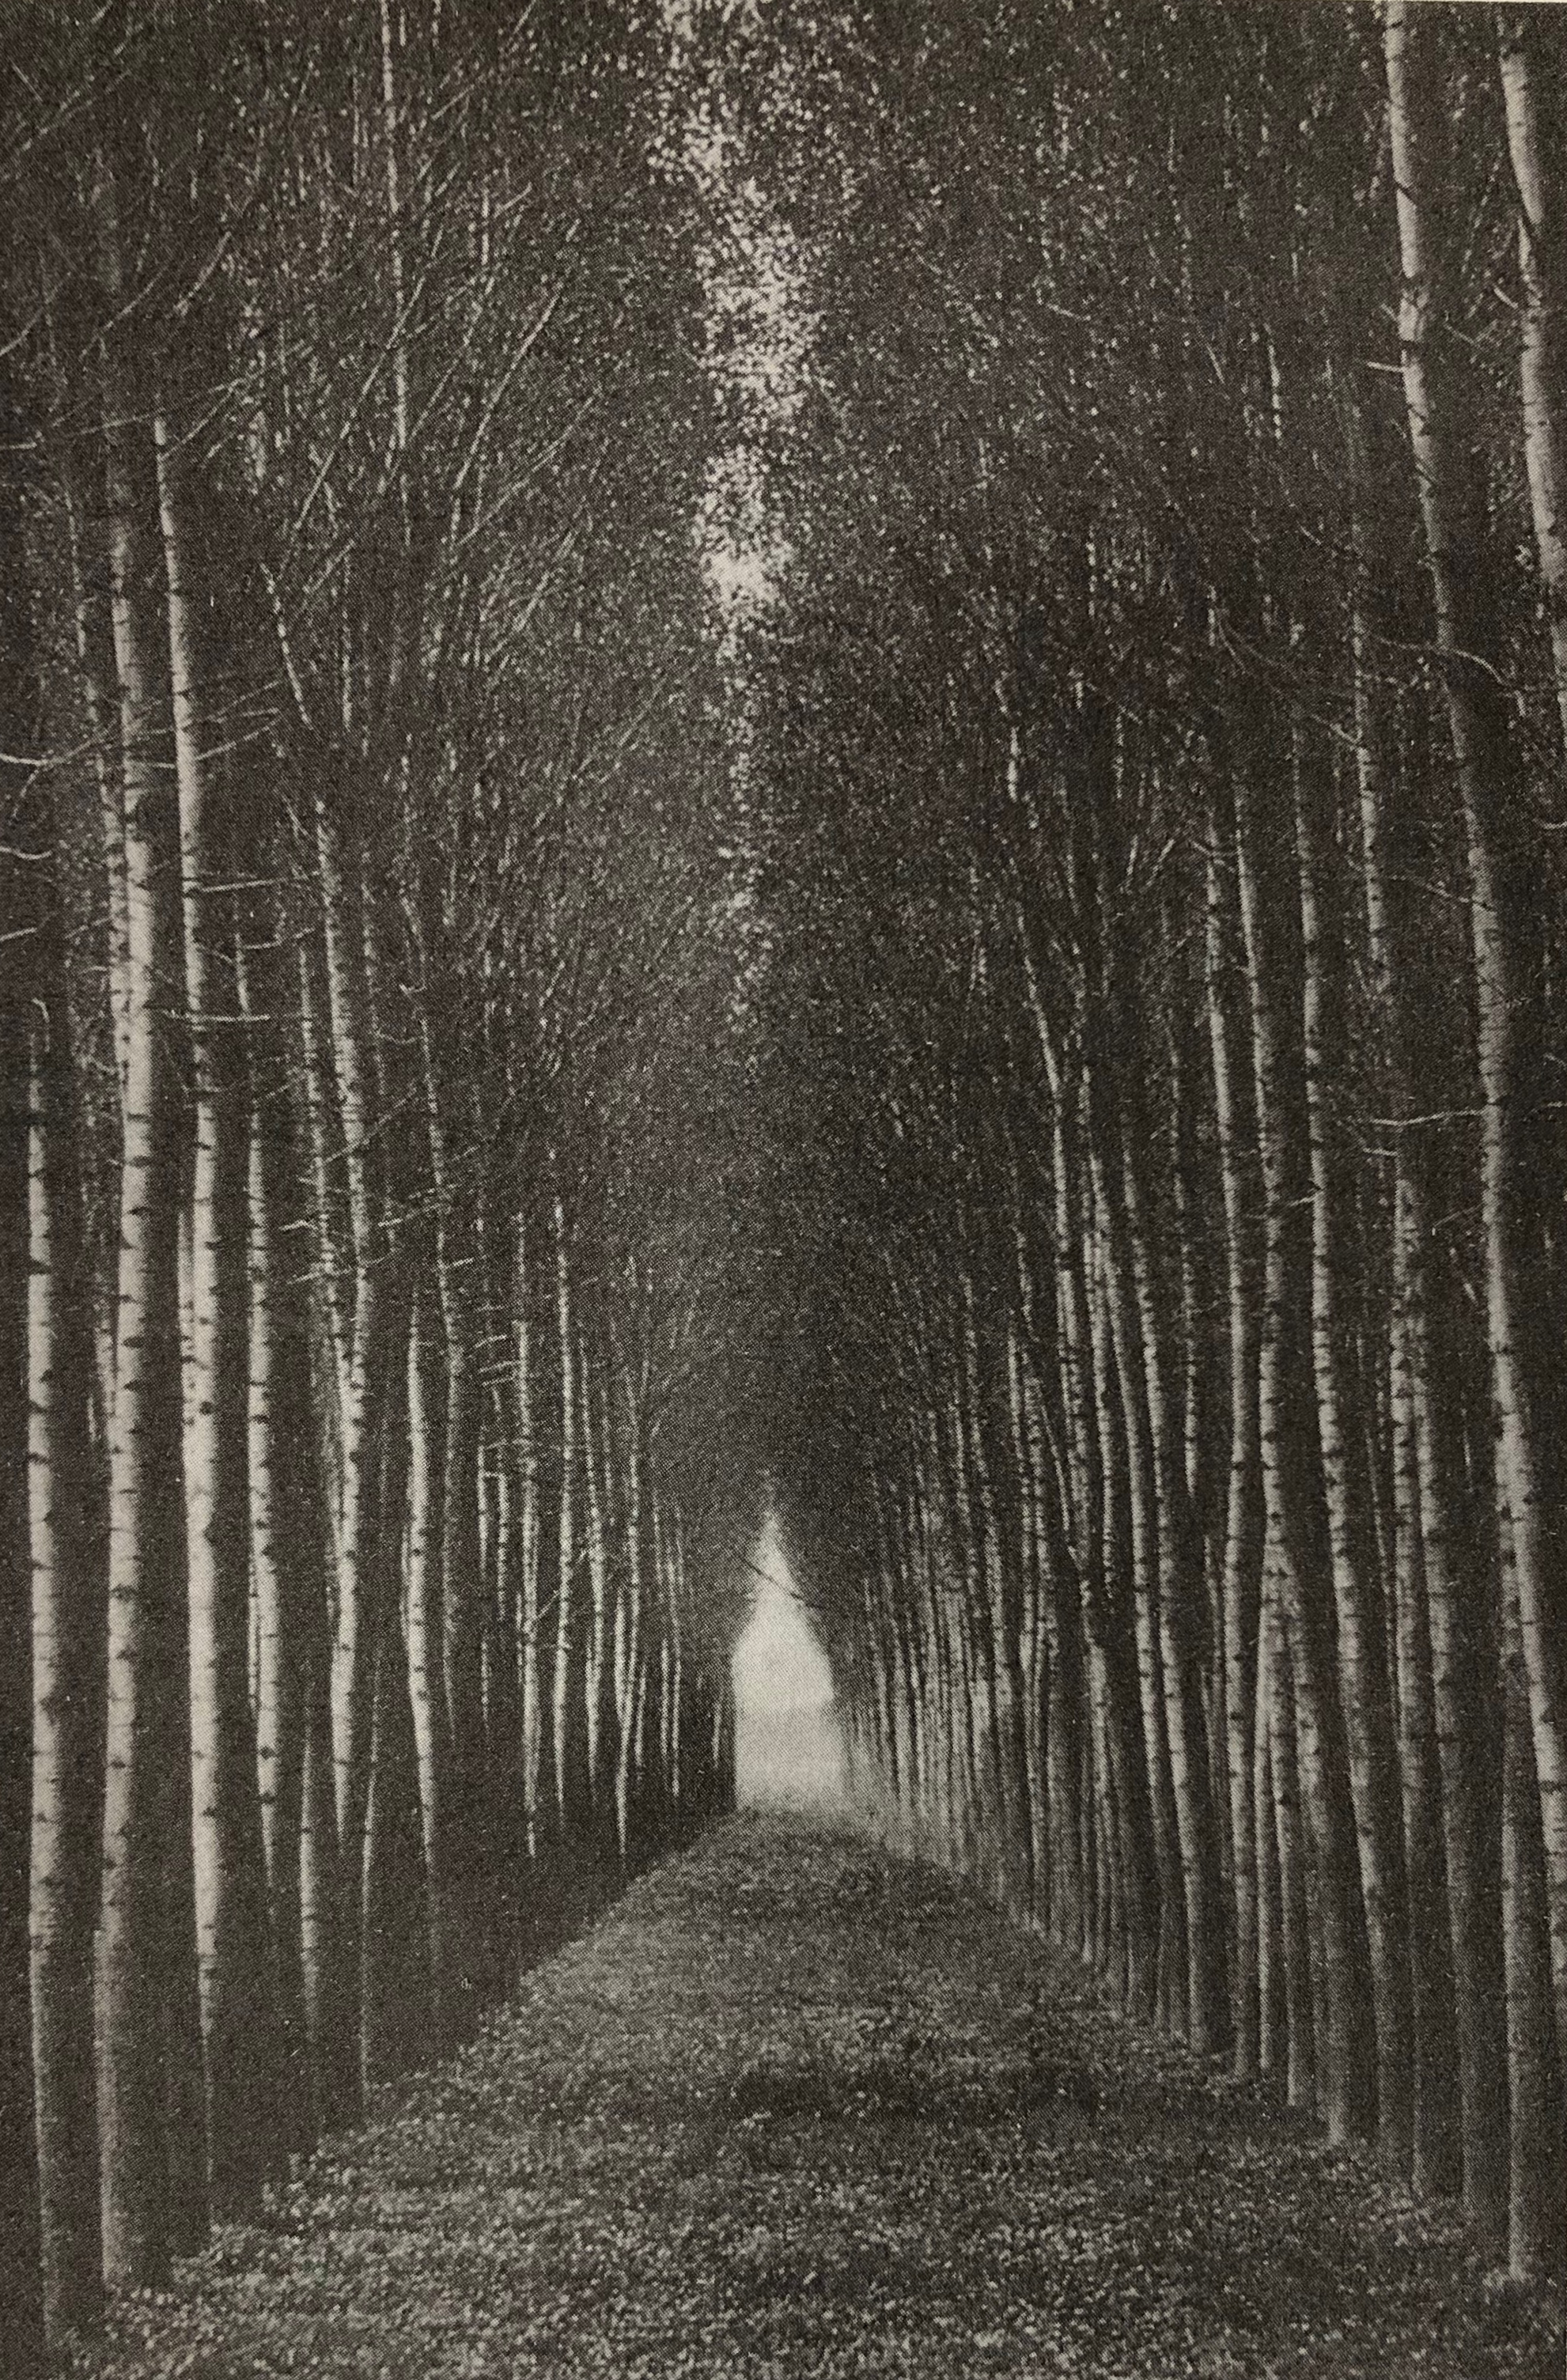
\includegraphics[height=\textheight]{figures/scifor.jpg}}
  \end{column}
  \end{columns}

\end{frame}


\begin{frame}[t]\frametitle{delayed disasters}
  \begin{itemize}
    \item things were fine for a while
    \item then they weren't
      \begin{itemize}
        \item pests
        \item storms
        \item lots of bad stuff
      \end{itemize}
  \end{itemize}

\vfill

\centering
\visible<2->{\textit{\LARGE Waldsterben}

\visible<3->{\textit{\large{Forest death}}}
}

\vfill

\end{frame}


\begin{frame}{ecological diversity}
  turned out we need all the stuff we removed from the forest.

\end{frame}


\end{document}